
\begin{document}

\chapter{Implementation}

\label{chapter:Implementation}

This chapter describes the development methodology, the source control
procedure, the initial implementation in Python, the final implementation in
C++ and the general structure and work-flow of the code.

\section{Development Methodology}

Since this project is primarily research, an agile development methodology was
used. There were no set requirements for the project, and instead the author
was encouraged to produce results towards a goal. The solution was devised by
determining a set of intermittent goals and possible solutions. As you can see
in Ch.~\ref{chapter:design}, four different solutions were designed and three
were implemented, each using a different approach to solve the problem at hand.
The development feedback loop worked by first listing the objectives and goals
for the project, i.e. generating safe paths through dynamic environments. Once
an algorithm was designed that the author was confident could solve this
problem, it was implemented and tested both quantitatively and qualitatively.
If the behaviour of the robot did not resemble the desired behaviour, the
solution was either augmented to possibly change the behaviour of the robot, or
a new solution was devised.

\section{Source Control}

As a method of storing and updating the codebase, source control was used. In
particular, GitHub was used to store the code, its revisions, releases, and
notes. Along with the main codebase, GitHub was used to store the scripts
created for running tests and experiments and kept track of the experimental
results during development. Only working and compilable code was pushed to the
Git repository and since there was only one developer, a continuous integration
server was not used. Instead, before a commit could be pushed to the server,
the code had to be compilable and pass a set of sanity checks. These sanity
checks consisted of checking whether roadmaps could still be generated and if
the basic operations on the data structures still functioned properly.

\section{Initial Implementation}

Due to the ease of development and the author's experience with the language,
Python was chosen as the initial language for the implementation. All three
attempts described in Ch.~\ref{chapter:design}, were implemented and a suite of
tests scripts and visualization mechanisms were created in order to
incrementally assess how each planner was behaving. However after the
implementation was completed for the final design described in
Sec.~\ref{sec:finaldesign}, it was discovered that Python could not produce
solution paths (without replanning) through dynamic environments in a real-time
scenario. Since Python could not search the graph within an acceptable amount
of time, it could only be used for \emph{a priori} planning and therefore could
not be used in stochastic environments in which replanning would be needed. Due
to this drawback, the author decided to rewrite the entire implementation in
C++.  Since this initial attempt is complete, it is publicly available
at~\cite{racer}.

\section{Final Implementation}

The final implementation was written in C++ due to the tremendous speed
improvement which made planning in real-time viable. Due to the object oriented
structure of C++, the planner and the associated data structures were
encapsulated in classes which made it very easy for people to use the code as
an API. While designing the software, extra effort was put into making the code
easily usable by other people who are not necessarily experts in robotics or
motion planning.  The system has an easy import mechanism and several examples
on how to use the different planners that have been implemented.

In order to visualize the paths that the planner has generated, the C++ code
can export the paths of the robot and the dynamic obstacles to a JSON file and
a Python script then can read and parse the generated JSON and display the
paths using either Matplotlib or RViz. Matplotlib is an open source library for
creating plots from data~\cite{matplotlib}. It is very similar to Matlab or
Mathematica except it runs natively in Python. RViz is a core component of the
Robotic Operating System (ROS) which can render dynamic scenes in three
dimensions and can visualize native geometrical and navigation messages from
ROS~\cite{ros}.  Since the paths are exported to JSON, a standard format with
parsers in many languages, third party software can be developed that can parse
the generated JSON file and analyze or visualize the generated paths.
Likewise, the Dodger library can be imported by a third party program to
control robots from the generated paths or to visualize the paths using other
visualization tools such as OpenGL. A diagram of this tool-chain is shown in
Fig.~\ref{fig:software}.

% change the below figure

\begin{figure}[h!]

    \centering

    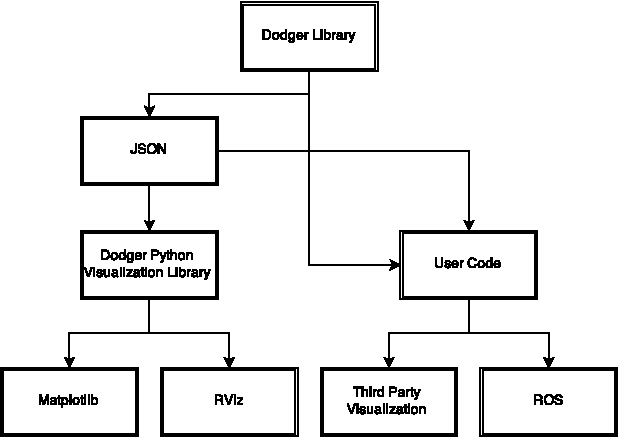
\includegraphics[width=0.8\linewidth]{figs/toolchain}

    \caption{A diagram depicting the work flow for the implementation. The
    Dodger library can either generate a path and export to a JSON file which
can then be visualized in Matplotlib or RViz using one of the Python scripts
provided or user code can read the exported JSON to control robots or visualize
the paths. The library can also be imported by user code to either visualize
paths or control a robot with ROS.}

    \label{fig:software}

\end{figure}

By separating the visualization code completely from the planner code, the
software is more easily portable to different visualization frameworks and
ensures that the user does not need to have a certain graphical software or ROS
installed for the software to be able to compile and use the library. This
allowed the planner code to be entirely self contained and simple to compile
with a provided CMake file which compiles the C++ code into a static library.
Likewise, this design decision in the implementation allows the generated paths
to be saved and either analysed or visualized at another time.  Also, since the
planner had no dependencies, experiments could be run on the servers provided
without needing root access.  This code is also made publicly available
at~\cite{dodger}.

\end{document}
